% Chapitre 2 — État de l'art (version française)

\chapter{État de l'art}

\section{Fondements du DNS}
\label{sec:2.1}

Le Système de Noms de Domaine (DNS) est l'annuaire distribué qui traduit les noms lisibles par l'humain en informations lisibles par machine --- principalement des adresses IP~\cite{RFC1034,RFC1035}. Sa hiérarchie reflète la délégation de l'autorité administrative sur des portions de l'espace de nommage : la zone racine délègue aux domaines de premier niveau (TLD), qui délèguent aux serveurs de noms faisant autorité pour les domaines individuels. La résolution est effectuée par un \textbf{résolveur récursif} agissant au nom des clients --- contactant successivement les serveurs racine, TLD et faisant autorité, et mettant en cache les résultats pour la durée du Time To Live (TTL) de chaque enregistrement.

Chaque enregistrement de ressource porte un TTL déterminant la durée de validité du cache. Les CDN utilisent des TTL courts (60~s ou moins) pour permettre une redirection rapide du trafic ; les enregistrements d'infrastructure stables portent des TTL de 24~heures ou plus. Pour la mesure active, deux implications en découlent : (1) interroger via un résolveur récursif peut retourner des réponses en cache périmées ; (2) la divergence d'état des caches entre sondes peut simuler des différences de routage géographique. Les requêtes directes aux serveurs faisant autorité contournent ces deux effets.

Le DNS stocke l'information sous forme d'\textbf{enregistrements de ressources} typés. Le tableau~\ref{tab:rr_types} liste les types pertinents pour ce mémoire. Les enregistrements \textbf{A} et \textbf{AAAA} sont les principaux observables : un domaine retournant des adresses IP différentes à différents points de mesure géographiques signale un routage CDN, une variation anycast ou une différenciation basée sur ECS. Les enregistrements \textbf{NS} identifient le fournisseur DNS ; l'analyse longitudinale des NS révèle les migrations de fournisseurs~\cite{vanRijswijk2016}. Les chaînes \textbf{CNAME} exposent l'opérateur CDN derrière un domaine. Les enregistrements \textbf{DNSKEY/DS/RRSIG} permettent de surveiller le déploiement DNSSEC, où des chaînes de clés de signature corrompues produisent des réponses \texttt{SERVFAIL} indiscernables d'une indisponibilité du serveur sans l'indicateur \texttt{CD} (Checking Disabled).

\begin{table}[tp]
\centering
\small
\begin{tabularx}{\linewidth}{p{1.4cm} p{3.6cm} l X}
\toprule
\textbf{Type} & \textbf{Contenu} & \textbf{Mesuré} & \textbf{Pertinence} \\
\midrule
A     & Adresse(s) IPv4                   & Primaire  & Observable principal : la variation géographique signale un routage CDN ou anycast \\
AAAA  & Adresse(s) IPv6                   & Primaire  & Parallèle à A ; le routage anycast peut différer entre protocoles~\cite{Bortzmeyer2013} \\
NS    & Noms des serveurs faisant autorité & Hebdo.   & Identifie le fournisseur DNS ; permet le suivi des migrations~\cite{Xu2023} \\
CNAME & Alias de nom canonique            & Dérivé    & Chaîne de délégation CDN ; la résolution révèle l'opérateur CDN \\
MX    & Nom(s) du serveur de messagerie   & Trimestr. & Suivi de l'adoption du courrier cloud~\cite{vanRijswijk2016} \\
SOA   & Enregistrement d'autorité de zone & Trimestr. & Le numéro de série permet la détection de changements \\
DNSKEY/DS & Clés/délégation DNSSEC      & Trimestr. & Surveillance du déploiement DNSSEC~\cite{vanRijswijk2016} \\
\bottomrule
\end{tabularx}
\caption{Types d'enregistrements de ressources DNS pertinents pour ce mémoire. Les types \textit{Primaires} sont inclus dans la campagne de mesure quotidienne.}
\label{tab:rr_types}
\end{table}

\section{Paradigmes de mesure DNS}
\label{sec:2.2}

Le \textbf{DNS passif} (pDNS) capture les requêtes et réponses aux résolveurs ou points d'échange existants sans injecter de trafic artificiel. Il reflète le comportement réel des utilisateurs et convient bien à la forensique de sécurité (suivi de botnets, détection de phishing via des services commerciaux comme Farsight DNSDB). Sa limitation fondamentale pour ce mémoire est la \textbf{cécité géographique} : un capteur passif n'observe que le trafic à son emplacement~\cite{vanRijswijk2016}. Il ne peut pas non plus mesurer un corpus de domaines prédéfini, et les contraintes de confidentialité (RGPD) limitent la granularité de conservation.

La \textbf{mesure DNS active} envoie délibérément des requêtes depuis des points de mesure contrôlés, permettant une couverture complète du corpus de domaines, un contrôle géographique et la reproductibilité. Van Rijswijk-Deij et al.~\cite{vanRijswijk2016} démontrent que même à 1,85 milliard de requêtes quotidiennes pour le TLD \textit{.com} seul, une mesure active bien cadencée ne représente que 0,3--1,6\,\% du trafic des serveurs faisant autorité --- un impact négligeable. Van der Toorn et al.~\cite{vanderToorn2018} exploitent 180 jours de telles données pour détecter le spam \textit{snowshoe} avec une précision supérieure à 93\,\% et 100 jours d'avance sur les listes noires, un résultat exclusif au paradigme actif.

\textbf{Cadre éthique} : Kisteleki et al.~\cite{Kisteleki2016} ancrent l'éthique des mesures RIPE Atlas dans le Rapport Menlo (2012) : les chercheurs portent la responsabilité du trafic que les hôtes de sondes génèrent. Pour ce mémoire, le corpus de domaines est tiré de domaines Tranco publiquement accessibles ; aucun contenu politiquement sensible n'est interrogé ; et la fréquence de mesure respecte les TTL DNS.

\textbf{OpenINTEL}~\cite{vanRijswijk2016}, développé à l'Université de Twente, mesure chaque domaine d'une zone TLD quotidiennement depuis \textbf{un seul point de mesure aux Pays-Bas}. Il couvre plus de 50\,\% de l'espace de nommage DNS mondial, stocke les résultats en Apache Avro/Parquet, et fonctionne en continu depuis mars 2015. Ses données longitudinales ont soutenu des études sur les défaillances de gestion des clés DNSSEC (USENIX Security 2017, Distinguished Paper Award), l'adoption des protections DDoS (IMC 2016), et la migration vers le courrier en nuage~\cite{vanRijswijk2018blog}. La couverture s'est étendue des TLD initiaux \textit{.com}/\textit{.net}/\textit{.org} (50\,\% de l'espace de nommage mondial) à tous les gTLD d'ici 2018, et la plateforme a reçu le Prix des Données de Recherche des Pays-Bas en novembre 2018~\cite{vanRijswijk2018blog}. Sa limitation explicite est l'architecture à point unique : qu'un domaine retourne des adresses IP différentes à des sondes au Japon, au Brésil ou en Afrique du Sud est invisible dans les données OpenINTEL --- la motivation principale de l'approche distribuée de ce mémoire.

\section{Mesure distribuée : RIPE Atlas}
\label{sec:2.3}

RIPE Atlas est un réseau de sondes matérielles hébergées par des bénévoles, offrant la diversité spatiale qu'OpenINTEL ne possède pas. En 2024, il comprend environ \textbf{12\,900 sondes actives dans 178 pays}, générant environ 1,3 milliard de résultats de mesure par jour~\cite{Nosyk2024}. Le DNS est un type de mesure natif : chaque sonde mesure en continu les 13 adresses de serveurs racine DNS, et les campagnes définies par les utilisateurs peuvent interroger n'importe quel domaine, type d'enregistrement et résolveur. Le tableau~\ref{tab:platforms} compare RIPE Atlas aux principales plateformes alternatives.

\begin{table}[tp]
\centering
\small
\begin{tabularx}{\linewidth}{p{2.6cm} r p{2.0cm} p{1.8cm} X}
\toprule
\textbf{Plateforme} & \textbf{Sondes} & \textbf{Pays} & \textbf{DNS natif} & \textbf{Notes} \\
\midrule
RIPE Atlas       & $\approx$12\,900 & 178 & Oui & Matériel bénévole ; système de crédits ; accès ouvert~\cite{Nosyk2024} \\
CAIDA Ark        & $\approx$170     & 60+ & Non & Axé topologie ; support DNS limité~\cite{Bajpai2017} \\
SamKnows         & $\approx$70\,000 & 50+ & Non & Déployé par ISP ; QoS haut débit ; non ouvert~\cite{Bajpai2017} \\
PlanetLab        & $\approx$300     & 60+ & Non & VMs logicielles ; largement inactif~\cite{Cicalese2015} \\
BISmark          & $\approx$420     & 40+ & Non & Axé réseau domestique ; diversité limitée~\cite{Bajpai2017} \\
\bottomrule
\end{tabularx}
\caption{Comparaison des plateformes de mesure Internet distribuées. RIPE Atlas est la seule plateforme avec un support DNS natif et un accès académique ouvert à l'échelle mondiale.}
\label{tab:platforms}
\end{table}

\textbf{Sélection des sondes} : Bajpai et al.~\cite{Bajpai2017} distinguent les \textit{balises système} (dérivées automatiquement des mesures intégrées de RIPE Atlas toutes les quatre heures, fiables) des \textit{balises utilisateur} (définies manuellement par les hôtes de sondes ; seulement 2,8\,\% les mettent à jour, les rendant souvent périmées). Le protocole de sélection recommandé est : filtrer par balises système (\texttt{system-ipv4-works}, \texttt{system-resolves-a-correctly}), puis stratifier géographiquement pour compenser la concentration à 91\,\% en Europe/Amérique du Nord. Holterbach et al.~\cite{Holterbach2015} documentent en outre une \textbf{interférence entre mesures} : les campagnes concurrentes sur les mêmes sondes introduisent des erreurs de temporisation de 1--7~ms et une désynchronisation temporelle allant jusqu'à une heure. La planification aux heures creuses et l'utilisation de mesures répétées atténuent ces deux effets.

\textbf{Biais géographique} : L'Allemagne et les États-Unis représentent ensemble 28\,\% de toutes les sondes ; l'Afrique, l'Amérique latine et l'Asie du Sud-Est sont substantiellement sous-représentées par rapport à leurs parts de la population d'utilisateurs Internet mondiale~\cite{Nosyk2024}. La figure~\ref{fig:ripe_atlas_distribution} cartographie cette distribution. La stratification géographique lors de la sélection des sondes est donc obligatoire pour toute étude de la variation DNS mondiale.

\begin{figure}[tp]
  \centering
  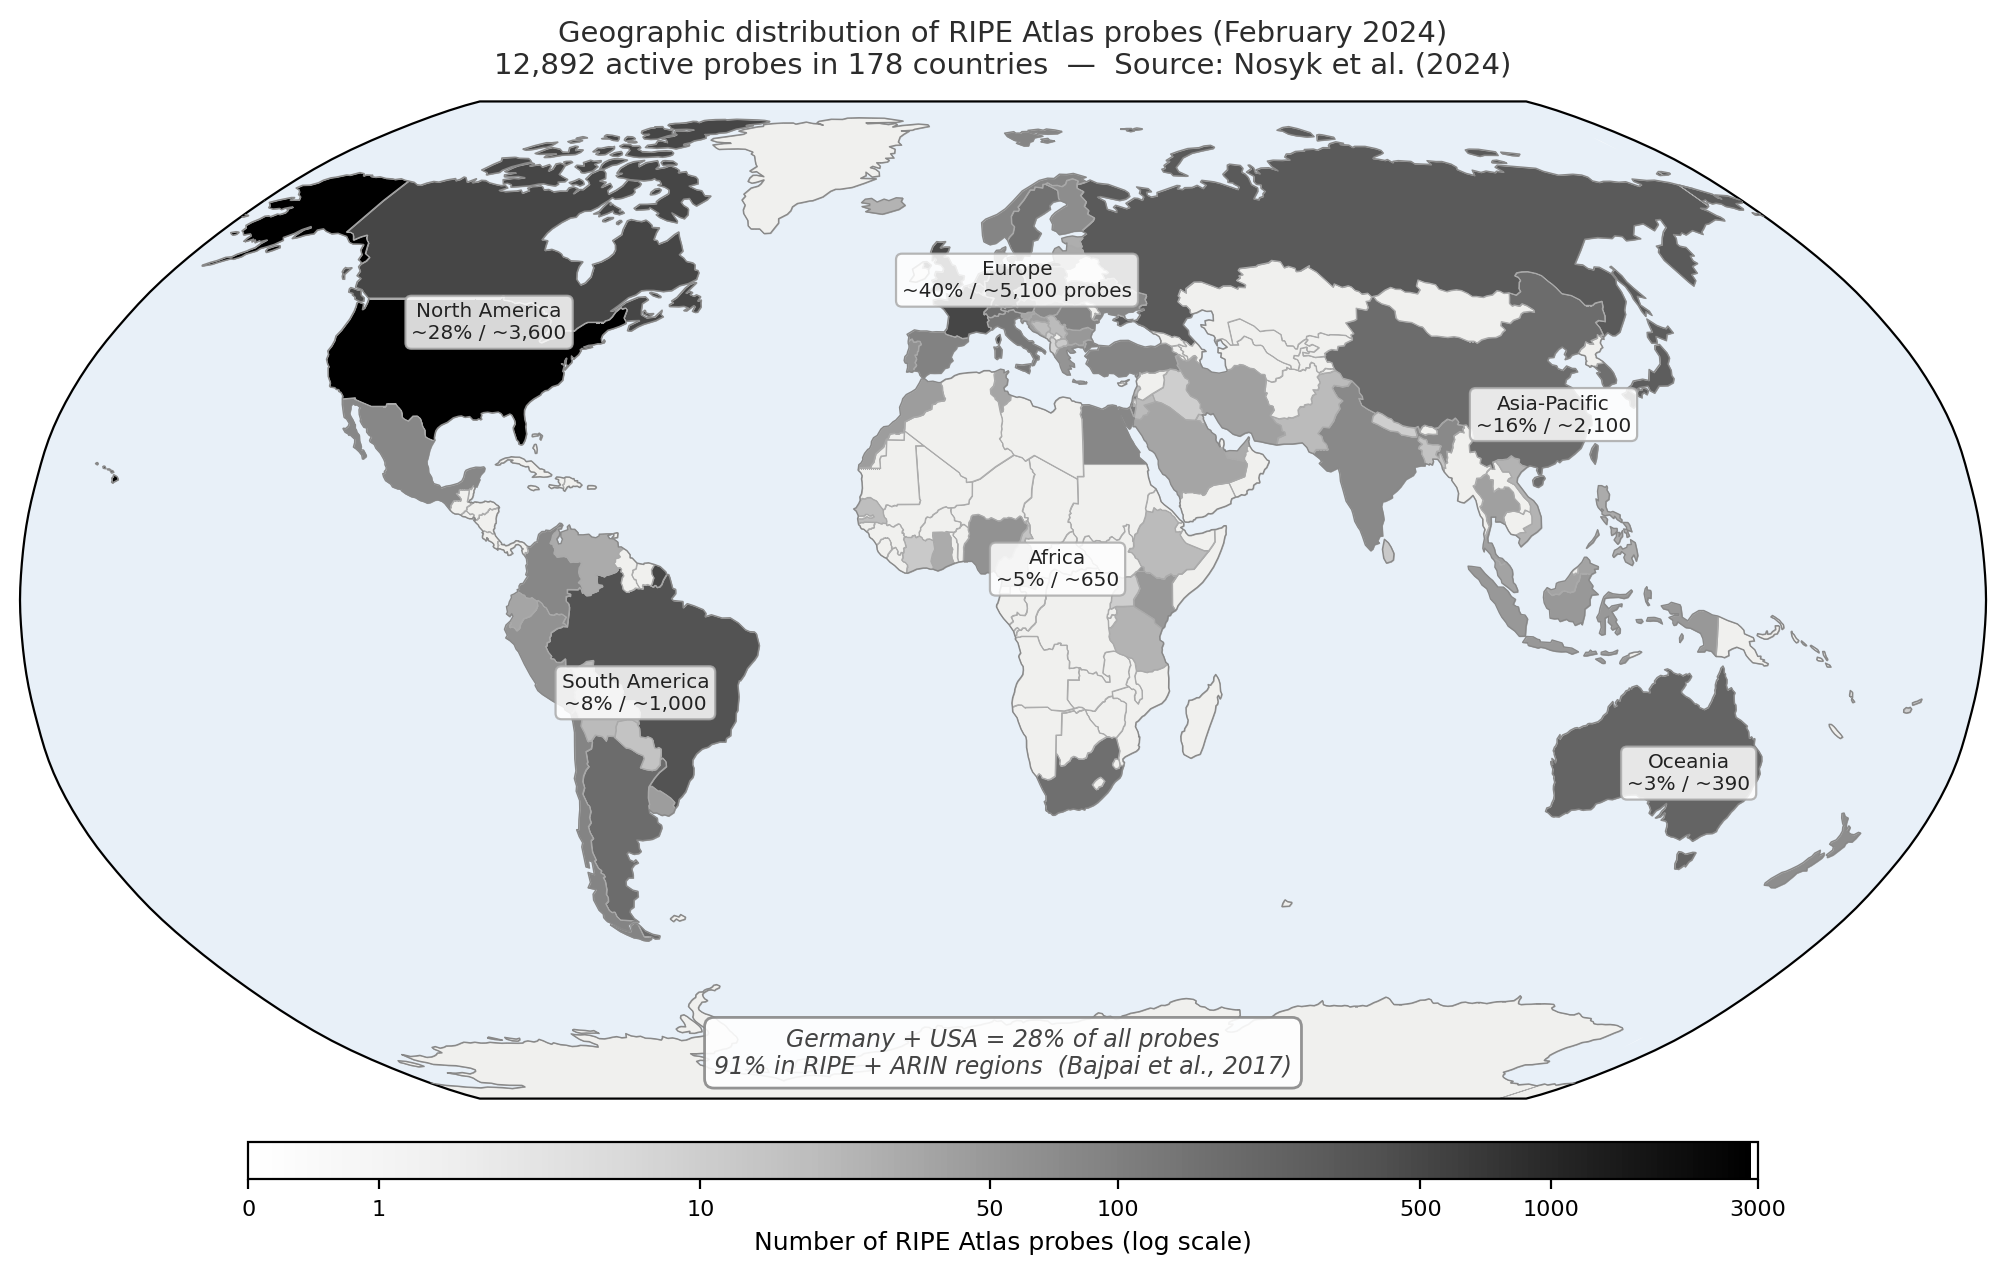
\includegraphics[width=0.90\linewidth]{figures/fig4_ripe_atlas_distribution.png}
  \caption{Distribution géographique des sondes RIPE Atlas (2024). L'Allemagne et les États-Unis représentent 28\,\% de toutes les sondes actives ; 91\,\% des sondes dual-stack sont dans les régions RIPE (Europe/Moyen-Orient) et ARIN (Amérique du Nord)~\cite{Bajpai2017,Nosyk2024}.}
  \label{fig:ripe_atlas_distribution}
\end{figure}

\textbf{Validité des mesures} : Jones et al.~\cite{Jones2016} détectent des proxies DNS transparents en chemin dans dix ISP : le proxy d'un ISP kenyan répond aux requêtes DNS racine 23$\times$ plus vite que le RTT ICMP réel vers le serveur B-root (14~ms vs 318~ms). Nosyk et al.~\cite{Nosyk2024} constatent que 69\,\% des sondes chinoises échouent à résoudre les domaines Meta --- un filtrage géographique, pas une défaillance de mesure. Ces résultats imposent deux étapes de contrôle qualité des données : vérifications de cohérence RTT pour identifier les sondes mandataires, et analyse croisée domaines/temps pour distinguer la censure des défaillances matérielles.

\section{Routage anycast dans le DNS}
\label{sec:2.4}

L'anycast IP est l'architecture de routage dominante pour les serveurs racine DNS, les serveurs TLD et les grands résolveurs publics (Google 8.8.8.8, Cloudflare 1.1.1.1). Les sondes situées dans différentes localisations géographiques peuvent contacter des serveurs physiquement différents derrière la même adresse IP anycast ; les réponses peuvent différer en latence et, dans certains cas, en contenu.

\textbf{Identification d'instance} : Deux techniques complémentaires permettent de localiser l'instance anycast qui a répondu à une requête. L'\textbf{option NSID} (RFC~5001) amène le serveur répondant à intégrer un identifiant dans sa réponse (par ex. \texttt{dns.th2.nic.fr} pour l'instance parisienne de d.nic.fr). La \textbf{requête CHAOS \texttt{id.server}} (RFC~4892) retourne un identifiant de code IATA (par ex. \texttt{ams}, \texttt{fra}) ; les enregistrements de classe CHAOS n'étant pas mis en cache, chaque requête atteint l'instance anycast routée par BGP en direct~\cite{Finnegan2018}.

\textbf{Bassins d'attraction BGP} : Bortzmeyer~\cite{Bortzmeyer2013} démontre pour d.nic.fr que la topologie de peering BGP, et non la géographie, détermine quelle instance anycast sert une requête. Les sondes nord-américaines routent 55\,\% de leur trafic vers l'instance parisienne et seulement 33\,\% vers Francfort --- malgré Paris étant $\approx$6\,000~km plus loin. Finnegan~\cite{Finnegan2018} confirme ce schéma pour UncensoredDNS avec 500 sondes Atlas. La figure~\ref{fig:bgp_attraction_basins} illustre ces bassins d'attraction.

\begin{figure}[tp]
  \centering
  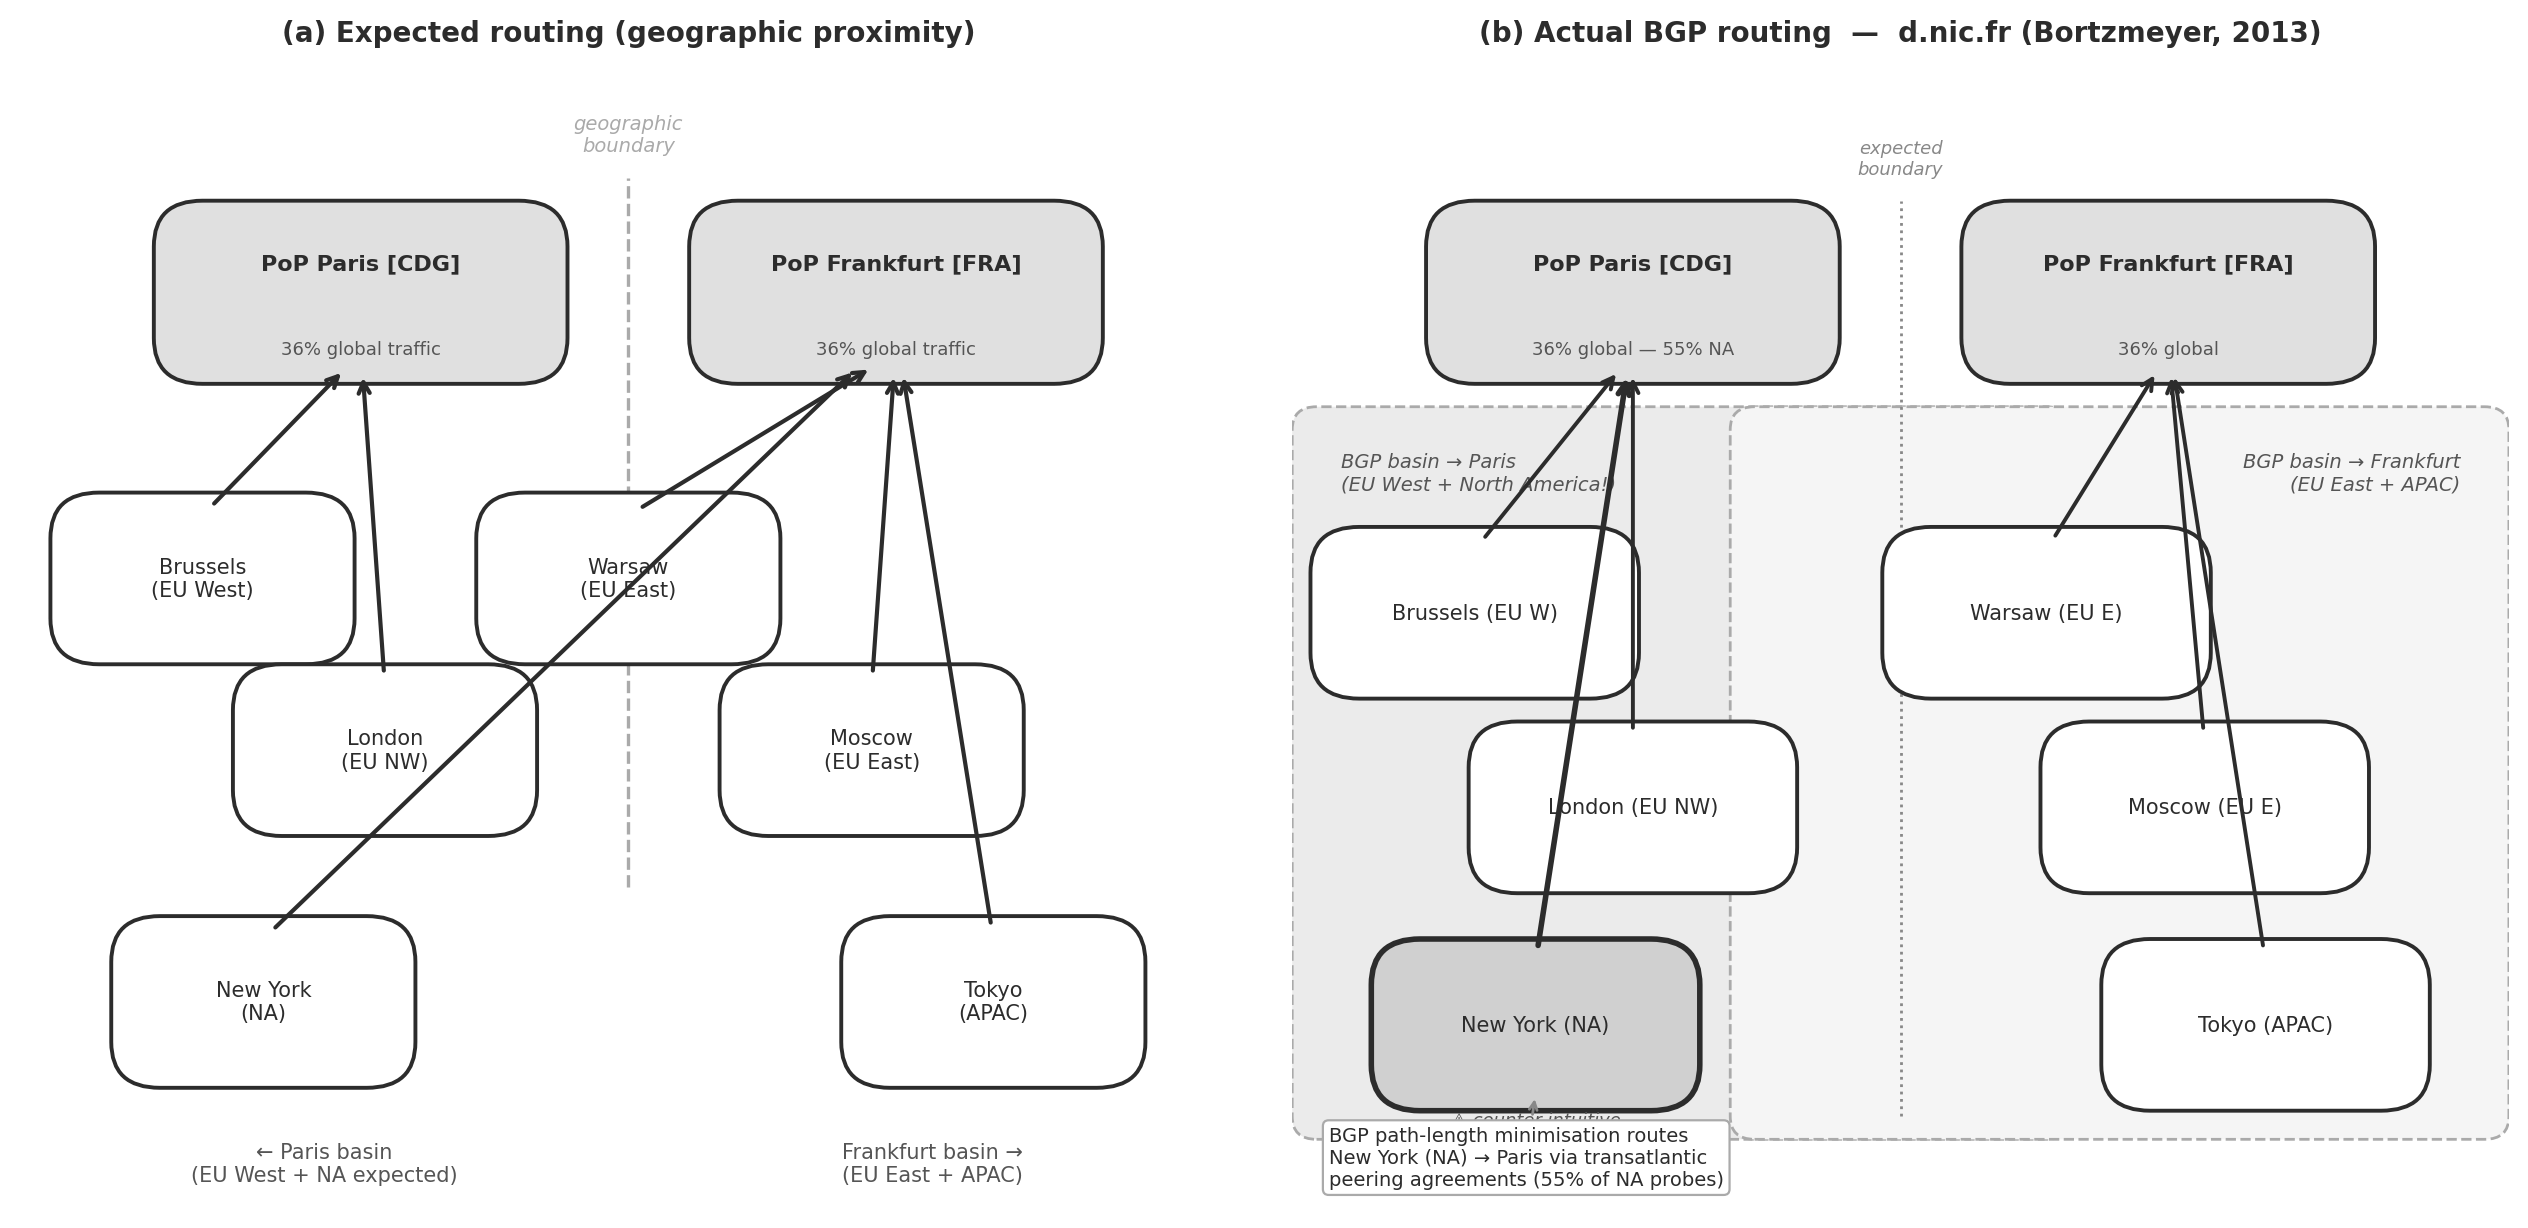
\includegraphics[width=0.92\linewidth]{figures/fig6_bgp_attraction_basins.png}
  \caption{Bassins d'attraction BGP pour d.nic.fr~\cite{Bortzmeyer2013}. Routage géographique attendu (a) vs routage BGP réel (b) : les sondes nord-américaines routent 55\,\% des requêtes vers Paris en raison des accords de peering BGP.}
  \label{fig:bgp_attraction_basins}
\end{figure}

\textbf{Divergence IPv4/IPv6} : Les tables de routage BGP IPv4 et IPv6 sont maintenues indépendamment. Bortzmeyer~\cite{Bortzmeyer2013} documente une inversion pour d.nic.fr : Francfort est l'instance IPv6 dominante (36\,\% des requêtes mondiales) mais subordonnée en IPv4 (17\,\%). Les mesures dual-stack doivent être menées et analysées séparément pour éviter de confondre les deux dimensions de routage. Koch et al.~\cite{Koch2021} montrent en outre que l'inflation anycast (routage vers une réplique sous-optimale) affecte plus de 95\,\% des utilisateurs pour au moins une lettre de serveur racine DNS, mais son impact pratique est négligeable pour le DNS racine car les enregistrements racine sont mis en cache pendant six jours.

\section{Routage CDN et EDNS Client Subnet}
\label{sec:2.5}

Les CDN utilisent le DNS comme mécanisme principal pour diriger chaque client vers un cluster de serveurs géographiquement approprié. Le serveur faisant autorité du CDN retourne un enregistrement A/AAAA différent selon la localisation inférée du résolveur interrogeant. Li et al.~\cite{Li2025}, étudiant Twitch, constatent une granularité de routage DNS CDN au niveau continental : des groupes d'adresses IP CDN distincts sont retournés aux sondes en Europe, Amérique du Nord et Asie-Pacifique, créant des frontières géographiques nettes détectables par mesure active distribuée.

\textbf{Le problème DNS distant} : Le routage CDN basé sur DNS suppose que le résolveur récursif est proche de ses clients. Lorsque les clients utilisent un résolveur public (Google 8.8.8.8, Cloudflare 1.1.1.1), le CDN perçoit la localisation du résolveur plutôt que celle du client. Hours et al.~\cite{Hours2016} quantifient cet effet causalement à partir de traces TCP passives d'un ISP : les clients utilisant Google DNS reçoivent des serveurs Akamai en moyenne 20~ms plus lointains en RTT, avec un effet secondaire de réduction du débit de 14\,\% dû à des fenêtres de congestion serveur plus petites. Wang et al.~\cite{Wang2018} constatent que l'adoption du DNS public croît de 27\,\% par an et que les inadéquations atteignent 113\,\% de distance serveur --- plus du double de l'assignation optimale.

\textbf{EDNS Client Subnet (ECS)}~\cite{RFC7871} résout ce problème en intégrant le préfixe /24 du client dans la requête transmise au serveur faisant autorité. Le CDN utilise ce préfixe (et non l'IP du résolveur) pour la sélection du serveur. ECS introduit un compromis de confidentialité : la localisation réseau du client devient visible pour le serveur faisant autorité et tout observateur en chemin. La RFC~7871 recommande de désactiver ECS par défaut. En pratique, Bortzmeyer~\cite{Bortzmeyer_tutorial} constate que la plupart des sondes RIPE Atlas utilisent des résolveurs qui ne transmettent pas ECS, donc les réponses sont généralement déterminées par l'IP du résolveur. Pour désactiver explicitement ECS, SOURCE PREFIX-LENGTH = 0 peut être défini dans la requête. La figure~\ref{fig:ecs_schema} illustre les trois scénarios ECS.

\begin{figure}[tp]
  \centering
  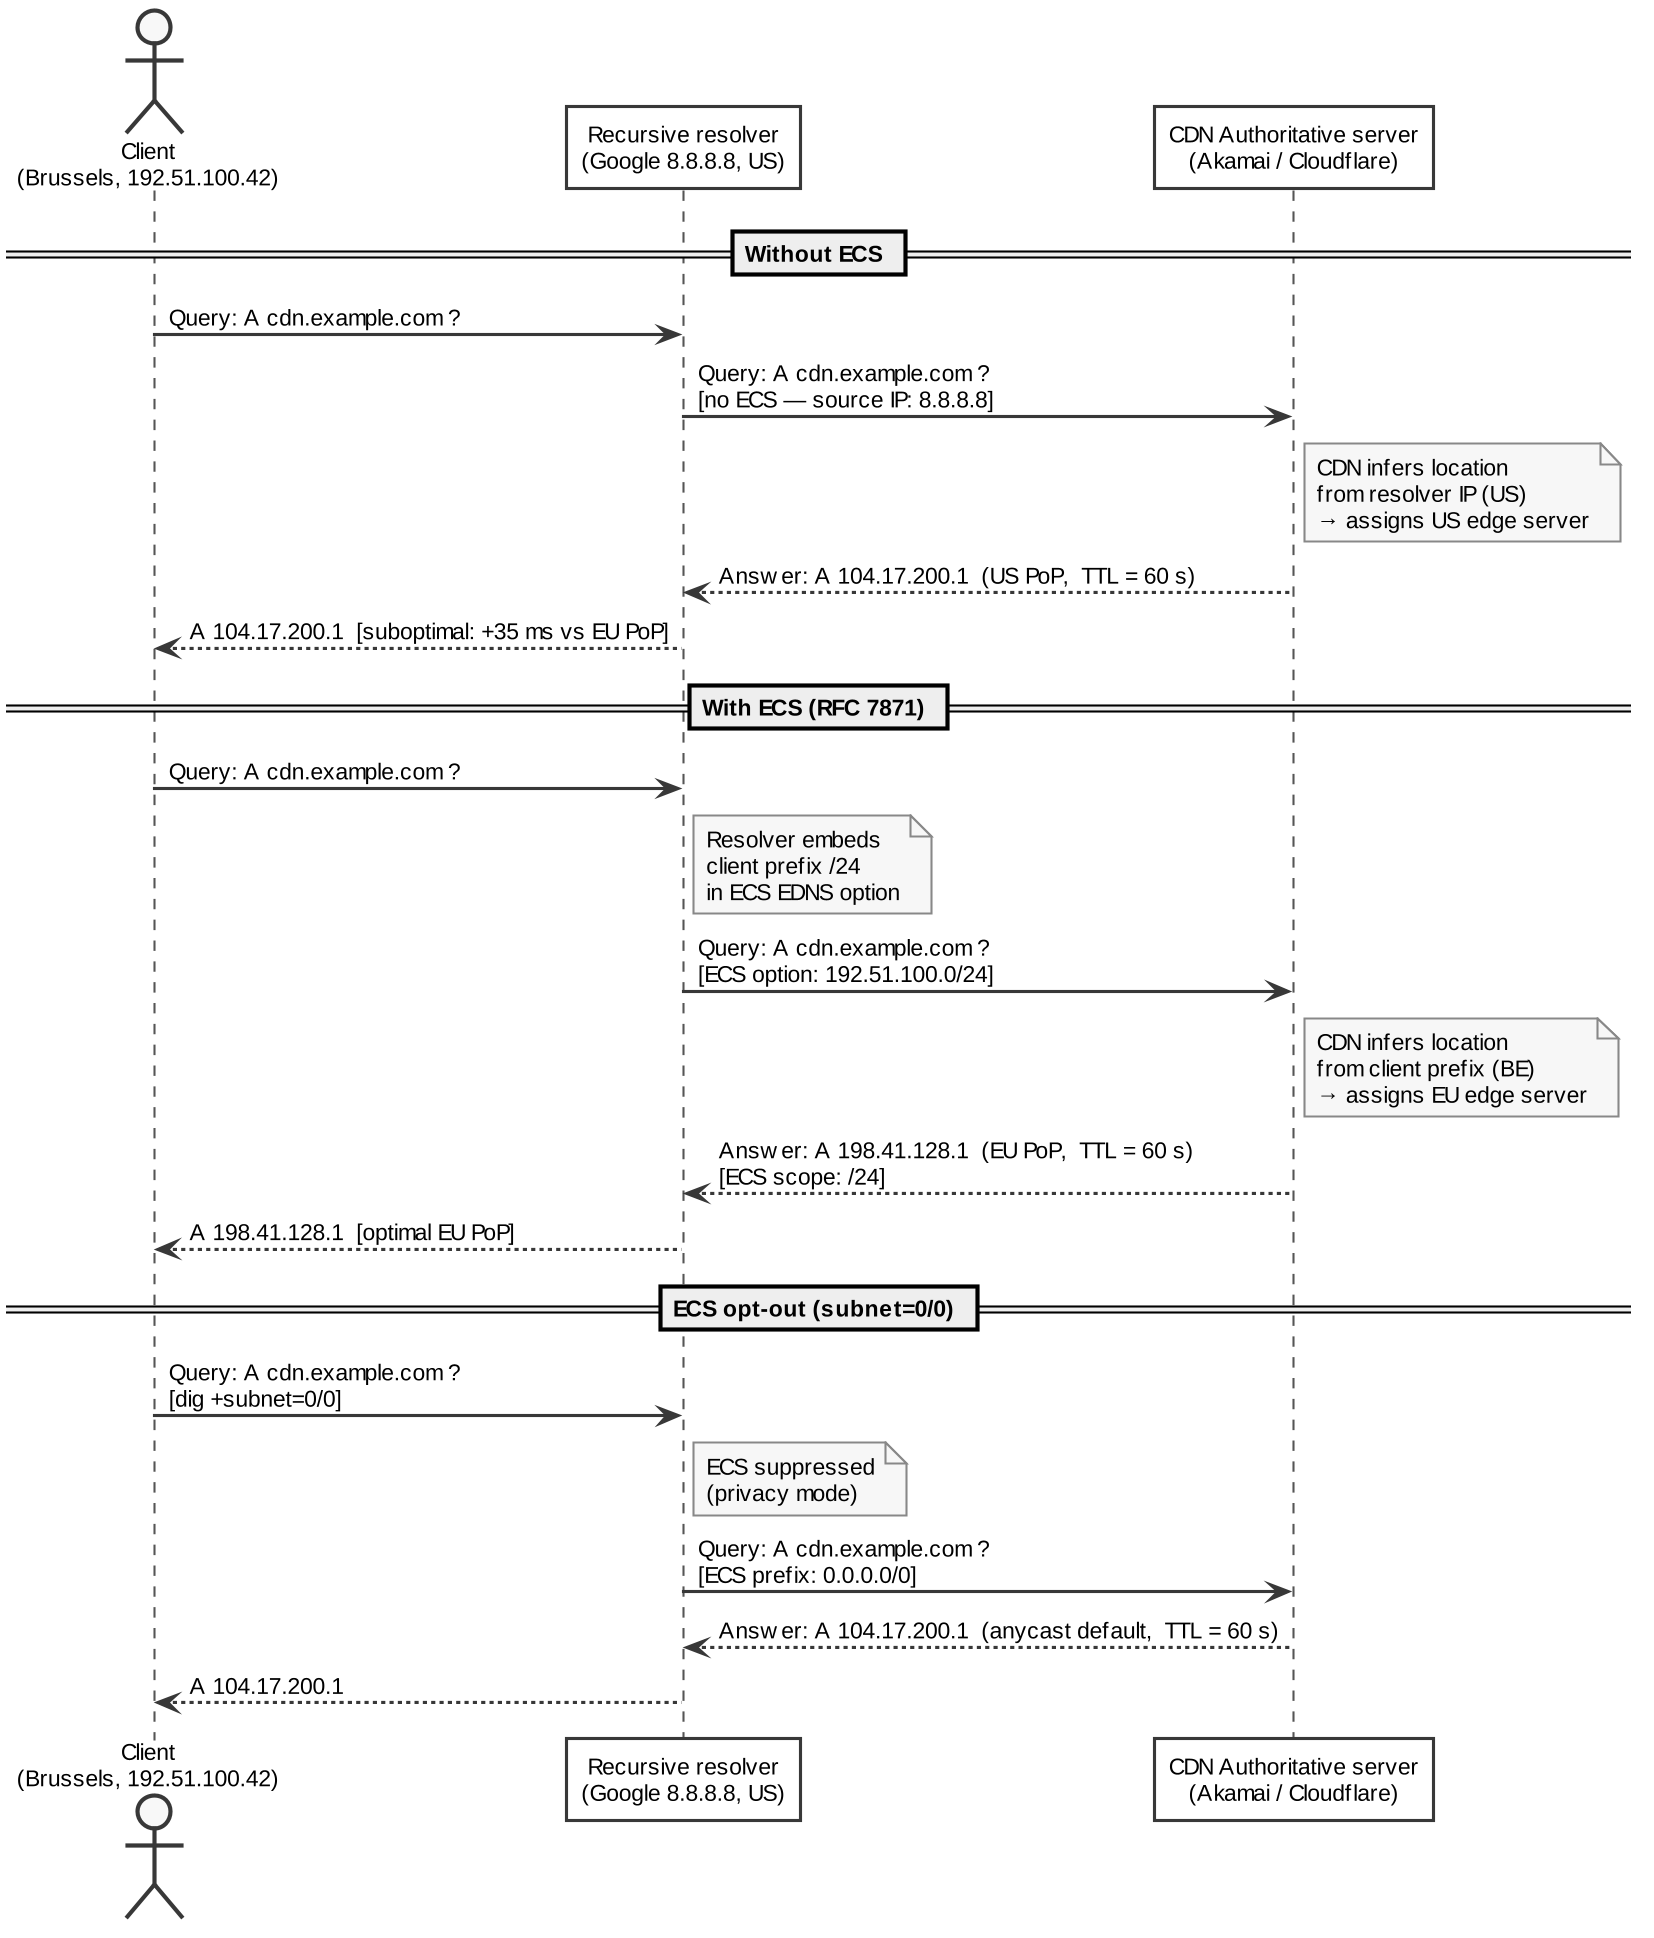
\includegraphics[width=0.90\linewidth]{figures/fig5_ecs_schema.png}
  \caption{Effet d'EDNS Client Subnet (ECS, RFC~7871) sur le routage géographique CDN. Sans ECS, le CDN utilise l'IP du résolveur (sous-optimal pour un client belge utilisant Google DNS). Avec ECS, le préfixe /24 du client guide la sélection du serveur. L'exclusion ECS (\texttt{subnet=0/0}) revient au routage par IP du résolveur.}
  \label{fig:ecs_schema}
\end{figure}

\textbf{Centralisation de l'infrastructure DNS} : Xu et al.~\cite{Xu2023} montrent que plus de 90\,\% des résolveurs de transfert sont soutenus par moins de 5\,\% des résolveurs récursifs indirects, et que seulement 10 fournisseurs DNS servent 48,5\,\% de tous les noms de domaine gTLD. La diversité géographique des sondes RIPE Atlas (chacune utilisant un résolveur ISP différent) est donc partiellement illusoire au niveau de la couche de résolution. Interroger directement les serveurs faisant autorité contourne cette centralisation cachée et constitue une exigence méthodologique de ce mémoire.

\section{Listes de classement de domaines}
\label{sec:2.6}

Les études du comportement DNS à grande échelle requièrent un corpus de domaines reproductible. Le Pochat et al.~\cite{LePochat2019} évaluent quatre listes de classement disponibles gratuitement --- Alexa, Cisco Umbrella, Majestic et Quantcast --- et constatent qu'elles ne se recoupent que sur $\approx$70\,000 des 2,82 millions de domaines uniques combinés (chevauchement pondéré par rang de 24--33\,\%). Le changement de méthodologie d'Alexa en 2018 a provoqué un renouvellement de 50\,\% de la liste quotidiennement, rendant les études longitudinales peu fiables. Cisco Umbrella contient $\approx$51\,\% d'entrées non-web (noms d'hôtes EC2, fautes de frappe). Majestic contient 2\,162 domaines malveillants documentés. Les quatre listes sont trivialement manipulables : une seule requête HTTP depuis un navigateur avec l'extension Alexa peut hisser un domaine au rang 28\,798. Le tableau~\ref{tab:ranking_lists} compare les principales propriétés.

\begin{table}[tp]
\centering
\small
\begin{tabularx}{\linewidth}{p{2.2cm} X X X X}
\toprule
\textbf{Propriété} & \textbf{Alexa} & \textbf{Cisco Umbrella} & \textbf{Majestic} & \textbf{Tranco} \\
\midrule
Source de données  & Extension navigateur & Requêtes DNS OpenDNS & Liens d'exploration web & Agrégation multi-sources \\
Taux chgt. quotid. & $\approx$50\,\% (post-2018) & $\approx$10\,\% & $\approx$1\,\% & $\approx$0,6\,\% \\
Effort manipulation & 1 req. HTTP & 1 injection req. DNS & Quelques backlinks & 4$\times$ vs source unique \\
Entrées non-domaine & Faible & $\approx$51\,\% & Faible & Filtrées \\
Domaines malveillants & Quelques-uns & Quelques-uns & 2\,162 documentés & Filtrés \\
Reproductibilité   & Écrasement quotidien & Écrasement quotidien & Écrasement quotidien & Lien permanent stable \\
\bottomrule
\end{tabularx}
\caption{Comparaison des listes de classement de domaines. Tranco est la seule liste conçue pour la reproductibilité de la recherche et la résistance à la manipulation~\cite{LePochat2019}.}
\label{tab:ranking_lists}
\end{table}

\textbf{Tranco}~\cite{LePochat2019} agrège plusieurs listes sur une fenêtre glissante de 30 jours par décompte de Borda, produisant un corpus stable (0,6\,\% de changement quotidien), résistant à la manipulation (effort quadruplé sur plusieurs listes), et reproductible via des liens permanents archivés. Pour ce mémoire, la stabilité de Tranco garantit que le même ensemble de domaines est mesuré sur 90 campagnes quotidiennes, permettant une comparaison temporelle pertinente.

\section{Synthèse et positionnement}
\label{sec:2.7}

La revue précédente révèle un manque clair à l'intersection de la profondeur temporelle d'OpenINTEL et de la diversité spatiale de RIPE Atlas. OpenINTEL fournit une mesure DNS quotidienne à l'échelle TLD depuis 2015, mais depuis un seul point néerlandais : la variation géographique est invisible. Les études DNS RIPE Atlas existantes sont principalement des études de cas à campagne unique, à domaines limités (quelques centaines de domaines, un seul instant). Aucune étude n'a caractérisé de manière systématique quelle fraction des domaines populaires retourne des réponses DNS géographiquement différenciées, quels mécanismes produisent cette différenciation, ou comment elle évolue sur des mois. Le tableau~\ref{tab:gap_analysis} formalise ce positionnement.

\begin{table}[tp]
\centering
\small
\begin{tabularx}{\linewidth}{p{2.8cm} p{3.5cm} p{3.8cm} X}
\toprule
\textbf{Dimension} & \textbf{OpenINTEL} & \textbf{RIPE Atlas (existant)} & \textbf{Ce mémoire} \\
\midrule
Couverture domaines  & Fichiers de zone TLD complets & Définis par l'expérimentateur & Tranco Top-10K (stable, reproductible) \\
Point de mesure      & Point unique (Pays-Bas) & $\approx$12\,900 sondes, 178 pays & Stratification multi-continents \\
Profondeur temporelle & Quotidien depuis mars 2015 & Campagnes uniques & Campagnes répétées sur 90 jours \\
Suivi anycast        & Non applicable & Études de cas (d.nic.fr, UncensoredDNS) & Systématique sur le corpus \\
Contrôle résolveur   & Résolveur central fixe & Résolveur local de la sonde & Requête directe faisant autorité \\
\bottomrule
\end{tabularx}
\caption{Positionnement de ce mémoire par rapport à l'infrastructure de mesure DNS existante sur cinq dimensions. Chaque ligne identifie un manque que ce travail adresse explicitement.}
\label{tab:gap_analysis}
\end{table}

Trois lacunes spécifiques motivent la contribution :

\textbf{Lacune~1 --- Absence de caractérisation géographique DNS à l'échelle de la population} : Les études de cas anycast individuelles (Bortzmeyer~\cite{Bortzmeyer2013} ; Finnegan~\cite{Finnegan2018}) et les études de routage CDN (Hours et al.~\cite{Hours2016} ; Li et al.~\cite{Li2025}) ciblent un service ou domaine à la fois. Aucune étude n'a mesuré quelle fraction du corpus de domaines populaires retourne des réponses géographiquement différenciées, ni quels mécanismes dominent à cette échelle.

\textbf{Lacune~2 --- La centralisation des résolveurs compromet la diversité des points de mesure} : Utiliser les résolveurs locaux des sondes crée une diversité géographique apparente qui disparaît au niveau de la couche de résolution (90\,\% des résolveurs de transfert $\rightarrow$ 5\,\% des résolveurs récursifs, Xu et al.~\cite{Xu2023}). L'interrogation directe des serveurs faisant autorité est la mesure corrective nécessaire, mais aucune des études de cas citées ne la documente comme choix de conception explicite.

\textbf{Lacune~3 --- Les études à campagne unique manquent les dynamiques temporelles} : Koch et al.~\cite{Koch2021} et Bortzmeyer~\cite{Bortzmeyer2013} reconnaissent que le routage BGP et les bassins de capture anycast des CDN changent dans le temps. Une campagne longitudinale de 90 jours est nécessaire pour caractériser la stabilité ou la volatilité de la différenciation géographique des réponses DNS.

Ce mémoire adresse ces trois lacunes en déployant un système de mesure qui interroge le Tranco Top-10K directement aux serveurs faisant autorité depuis $\approx$100 sondes RIPE Atlas géographiquement stratifiées, répété quotidiennement sur 90 jours, avec suivi d'instances anycast par NSID et résultats archivés en Avro/Parquet selon les principes FAIR.
